\chapter{Giới thiệu}
Mạng nơ ron sâu (DNNs) đã đạt hiệu quả rất tốt với các bài toán trong học máy
và trí tuệ nhân tạo như phân loại ảnh, nhận diện giọng nói, dịch máy và trò chơi.
Mặc dù DNNs rất hiệu quả nhưng mốt số nghiên cứu gần đây đã chứng minh DNNs rất 
dễ  "tổn thương" với các mẫu đối nghịch (Szegedy et al. 2013; Goodfellow, Shlens, 
and Szegedy 2015). Ví dụ, một hình ảnh với nhiễu được thiết kế cẩn thận có thể
làm cho một DNNs đã được huấn luyện phân loại sai. Tệ hơn nữa, các mẫu đối nghịch
được tạo ra hầu như không thể phân biệt được bằng mắt người. 
\begin{figure}[H] % places figure environment here   
    \centering % Centers Graphic
    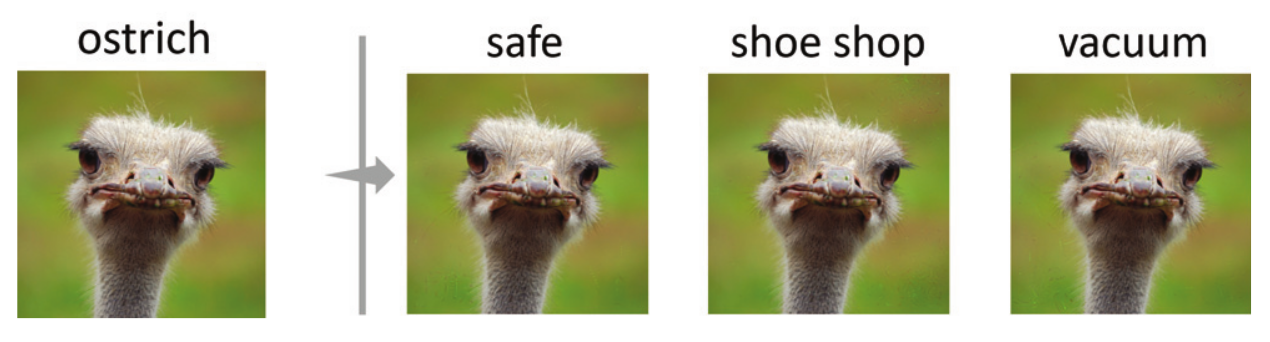
\includegraphics[width=0.8\textwidth]{assets/fig_01.png} 
    \caption{Minh họa trực quan về mẫu đối nghịch được sinh bởi EAD. 
    Hình gốc (đà điểu) được lấy từ tập ImageNet. Các mẫu đối nghịch bị 
    phân loại sai với mô hình Inception-v3.} % Creates caption underneath graph
    \label{fig:fg_01}
\end{figure}
Ví dụ trực quan trên thể hiện 3 mẫu đối nghịch của một hình con đà điểu ("ostrich") 
được sinh ra bằng thuật toán của chúng tôi. Các mẫu này được mô hình Inception-v3 
(Szegedy et al. 2016) phân loại thành "safe", "shoe shop" và "vacuum". \\

Sự thiếu mạnh mẽ của DNNs thể hiện trước các mẫu đối nghịch đã làm dấy lên những lo ngại 
nghiêm trọng về vấn đề bảo mật các ứng dụng, bao gồm nhận dạng tín hiệu giao thông 
và phát hiện phần mềm độc hại. Hơn nữa, vượt ra ngoài không gian kỹ thuật số, 
các nhà nghiên cứu đã chỉ ra rằng những mẫu đối nghịch này vẫn có hiệu quả trong thế giới 
vật chất trong việc đánh lừa DNNs (Kurakin, Goodfellow, and Bengio 2016a; Evtimov et al. 2017).
Do tính mạnh mẽ và ý nghĩa bảo mật, các phương tiện tạo ra các mẫu đối nghịch được gọi là 
các cuộc tấn công (\textit{attacks}) vào DNNs. Cụ thể, các cuộc tấn công có chủ đích 
(\textit{targeted attacks}) nhằm mục đích tạo ra các mẫu đối nghịch được phân loại nhầm thành các lớp mục tiêu 
cụ thể và các cuộc tấn công không có mục tiêu (\textit{untargeted attacks}) nhằm mục đích 
để tạo ra các mẫu đối nghịch không được phân loại như lớp học ban đầu. Các cuộc tấn công 
chuyển giao (\textit{transfer attacks}) nhằm mục đích tạo ra các mẫu đối nghịch có thể chuyển 
từ mô hình DNN này sang mô hình DNN khác. Ngoài việc đánh giá mức độ mạnh mẽ của DNNs,
Các mẫu đối nghịch có thể được sử dụng để huẩn luyện một mô hình mạnh có khả năng chống chịu 
với những xáo trộn của đối nghịch, được gọi là huấn luyện đối nghịch (\textit{adverarial training}) 
(Madry et al. 2017). Chúng cũng có được sử dụng để giải thích DNNs (Koh và Liang 2017;
Dong et al. 2017). \\

Trong bài báo này, chúng tôi sử dụng các mẫu đối nghịch để tấn công phân loại ảnh dựa trên 
mạng nơ ron tích chập. Mẫu đối nghịch được tạo ra để làm sai lệch kết quả dự đoán và phải đảm bảo
hình mới tạo ra giống với hình gốc. Trong quá khứ, sự giống nhau giữa mẫu đối nghịch được tạo
ra và hình gốc được đo bằng các tham số độ méo (\textit{distortion metrics}) khác nhau.
Một metric thường được sử dụng là chuẩn $L_q$ 
với $\lVert x \rVert_q = \left( \sum_{i=1}^p |x_i|^q \right)^{\frac{1}{q}}$ kí hiệu chuẩn $L_q$
của vector $p$ chiều $x = [x_1, ..., x_p]$ với $q \geq 1$. Đặc biệt, khi tạo ra các mẫu đối nghịch
, độ méo $L_{\infty}$ được sử dụng để đánh giá sự thay đổi tối đa giá trị pixel (Goodfellow, 
Shlens, and Szegedy 2015), trong khi độ méo $L_2$ được sử đụng để cải thiện chất lượng hình 
ảnh (Carlini and Wagner 2017b). Tuy nhiên, trong thực tế, chuẩn $L_1$ được sử dụng rộng rãi 
trong các bài toán phục hồi ảnh (Fu et al. 2006) cũng như phục hồi tính thưa (Candès and Wakin 2008),
Các mẫu đối nghịch dựa trên $L_1$ chưa được xem xét một cách kĩ càng. Trong bài toán mẫu đối nghịch,
độ biến dạng $L_1$ đánh giá tổng các thay đổi trong nhiễu loạn và đống vai trò là một thành phần
(hàm) lồi đo lường số lượng pixel thay đổi (độ thưa) gây ra bởi nhiễu. Để lấp đầy khoảng trống
này, chúng tôi xem xét một thuật toán tân công dựa trên hiệu chỉnh \textit{elastic-net}, được 
gọi là tấn công elastic-net vào DNNs (elastic-net attacks to DNNs - EAD). Hiệu chỉnh 
elastic-net là tổ hợp tuyến tính của các hàm penalty $L_1$ và $L_2$ và nó cũng là công cụ 
tiêu chuẩn cho bài toán lựa chọn tính chất đặc trưng cho dữ liệu nhiều chiều (Zou and Hastie 2005). 
Trong bài toán tấn công DNNs, EAD mở ra hướng nghiên cứu mới từ cách tân công hiện đại dựa trên 
$L_2$ (Carlini and Wagner 2017b) và cũng đề xuất tấn công hiệu quả hơn theo định hướng $L_1$
so với các phương pháp tấn công hiện có. \\

Để khám phá hiệu quả của tấn công dựa trên $L_1$, chúng tôi tiến hành các thử nghiệm trên tập 
dữ liệu MNIST, CIFAR10, và ImageNet trong các tình huống tấn công khác nhau. So sánh với các 
phương pháp tấn công hiện có dựa trên $L_2$ và $L_{\infty}$ (Kurakin, Goodfellow, and 
Bengio 2016b; Carlini and Wagner 2017b), EAD có thể đạt được tỉ lệ tấn công thành công tương 
tự khi phá vỡ DNNs được phòng thủ hoặc không phòng thủ (Papernot et al. 2016b). Quan trọng 
hơn, chúng tôi chỉ ra rằng, tấn công $L_1$ đạt được hiệu suất vượt trội so với các cuộc tấn
công $L_2$ và $L_{\infty}$ trong các cuộc tấn công chuyển giao với các mẫu đổi thủ được huấn
luyện bổ sung. Với tập dữ liệu khó nhất (MNIST), các kết quả từ EAD cải thiện tấn công chuyển 
giao vào DNN không được phòng thủ hay được phòng thủ đạt tỉ lệ thành công gần $99\%$. Thêm vào 
đó việc huận luyện kèm theo với mẫu đối nghịch dựa trên $L_1$ và $L_2$ có thể tăng cường khả 
năng phục hổi của DNNs đối với các nhiễu loạn. Những kết quả này gợi ý rằng EAD mang lại tập 
mẫu đối nghịch khác biệt nhưng hiệu quả hơn. Hơn thế nữa, đánh giá các cuộc tấn công dựa trên 
độ méo $L_1$ cung cấp thêm hiểu biết mới về học máy đối kháng và sự bảo mật của DNNs, gợi 
ý rằng $L_1$ có thể bổ sung cho $L_2$ và $L_{\infty}$ thúc đẩy các framework về học máy đối 
kháng hoàn thiện hơn.
